\documentclass{article}
\usepackage{epsfig,amsmath,amsfonts}
\usepackage{colortbl}
\usepackage{amsthm} % defines \begin{proof}

% \usepackage{graphicx} % I didn't have this, but may need it for graphicspath
\graphicspath{{.}{./figures/}}

% Question and TODO commands; leave just one of each pair uncommented
\newcommand{\TODO}[1]{{\color{red}{\bf TODO:} #1}}
\newcommand{\Question}[1]{{\color{red}{\bf Question:} #1}}
\newcommand{\Answer}[1]{{\color{cyan}{\bf Answer:} #1}}
%\newcommand{\TODO}[1]{}
%\newcommand{\Question}[1]{}
%\newcommand{\Answer}[1]{}
\newcommand{\comment}[1]{}  % Use this to comment out text, maybe many lines.
\newcommand{\Fmin}{F_{h-}}
\newcommand{\Fmax}{F_{h+}}
\newcommand{\shortcaption}{} % redefined below

\newtheorem{theorem}{Theorem}


\begin{document}

This document contains results and proofs for polynomial histograms,
for inclusion in a longer version of the paper.
This builds on Section~2.1 in the shorter paper (3 pages) polyhist.tex

\section{Introduction}

Material from polyhist.tex omitted here.

\section{Background}

Material from polyhist.tex omitted here.


\subsection{Information Loss Due to Binning}

Binning of an empirical
distribution into a histogram representation introduces a form of
preprocessing that constrains all later analyses based on that data
\cite{blocker2013potential}.  Bin breakpoints are often fixed in
advance for specific system quantities to reduce the computational
overhead of keeping track of many different histograms.
However, bin breakpoints that are
poorly chosen relative to the underlying data set may introduce
considerable error when one tries to compute means or percentiles
based on the histogram representations.  This is especially true for
the exponentially bucketed (e.g. buckets that double in size)
representations of distributions such as
latencies or arrival times that have a large dynamic range.

We will define an information loss metric based on
Earth Mover's Distance (EMD).
The EMD between
two distributions is the distance that mass must be moved to make
the distributions the same; in the one-dimensional case this is
\begin{equation}
  \mbox{EMD}(F,G)
  = \int_0^1 |F^{-1}(u) - G^{-1}(u)| du
  = \int_{-\infty}^\infty |F(x) - G(x)| dx
\end{equation}
where $F$ and $G$ are the two distribution functions.
This is also know as the first Mallow's
distance and first Wasserstein distance.
In the special case that one distribution is stochastically greater,
say $F(x) \ge G(x)$, then this reduces to $E_G(X) - E_F(X)$ if either
mean exists.

\Question{I didn't think about that earlier. Can we make use of that?}

We now apply that distance to measuring the information loss of a histogram
representation.
We define the
\emph{Earth Mover's Distance of the Cumulative Curves} (EMDCC)
as the largest possible EMD between distributions that are consistent
with a histogram.

To be definite,
suppose that random variable $X$ has
distribution $F$, and let
$F_{-}(x) = P(X < x)$ be the left-continuous version of $F$.
$F$ and $F_{-}$ differ at points of discontinuity.
% and $\mbox{EMD}(F, F_{-}) = 0$.
Let $h$ represent some information about the distribution of $X$,
such as a histogram.
Let $\Fmin(x)$ and $\Fmax(x)$ be the smallest and largest possible values
for $F_{-}(x)$ and $F(x)$, respectively, that are consistent with $h$.
% Emacs macros defined above:
% \Fmin = F_{h-}
% \Fmax = F_{h+}
% \Fminus = F_{-}
The EMDCC is the $L_1$ distance between $\Fmin$ and $\Fmax$,
\begin{equation}
  \mbox{EMDCC}(h)
  = EMD(\Fmin, \Fmax)
\end{equation}


\Question{The previous version normalized this.
Do we care about normalized? Is that standard?
Normalization introduces technical difficulties.
}

When $h$ is a histogram bucketing scheme,
$\Fmin$ puts its mass on the right endpoints and
$\Fmax$ on the left endpoints.
% (except for values of $x$ at boundaries; these discrepancies are
% of width 0 and have no effect on our metrics).

Figure~\ref{fig:emdcc} shows a histogram (left) along with the CDF representation and the
associated area of uncertainty (in yellow).  Any underlying dataset
having the given histogram representation must have a true ecdf lying
entirely within the yellow area.
The EMDCC is the sum of the areas of the yellow regions.
A histogram with more granular
buckets would reduce the information loss at the expense of additional
storage space to store the buckets.
Splitting each bucket in half would reduce EMDCC by half.

\begin{figure}[h!]
\centering
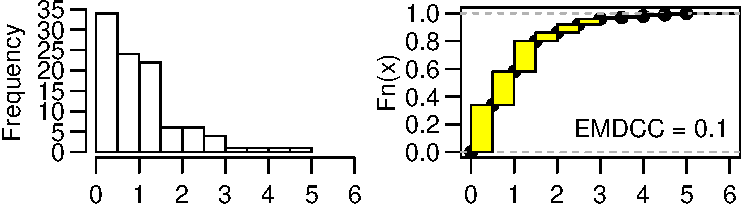
\includegraphics[width=\linewidth]{exhists-crop.pdf}
\caption{An example histogram (left);
 with its CDF representation and a
  yellow area of uncertainty showing where the true empirical cdf of
  the unbinned data must lie (right).}
\label{fig:emdcc}
\end{figure}

\TODO{Make that figure taller.
Can use smaller cex and mex
In the left figure, do tick labels at  0, 10, 20, ... (skip 5, 15, ...).
}
\TODO{Remove the dots in the right figure?
Or do they correspond to the CDF representation?
If so, make that clear, and improve the figure by redoing the dots after the
yellow rectangles are drawn.
}


\subsection{Polynomial Histograms}

Given a fixed amount of storage space, we can trade off the granularity of
histogram buckets for additional statistics within each bucket.  For example,
in addition to storing the counts between histogram boundaries $(a, b)$, we
could also store the mean and higher moments.  Histograms with
annotations of moments per bin are known as \emph{Polynomial
Histograms} \cite{sagae1997bin}.  Storing the moments is appealing in
a distributed systems context because merging histograms with the same
bucket boundaries remains trivial.

Knowing the first moment can help a lot when it is near a boundary; the
EMDCC associated with a bucket is zero if the mean is at either boundary.
Similarly, given the mean, knowing the variance can help a lot when
the variance is particularly small (the mass is concentrated near the mean)
or large (the mass is near the endpoints).

We will use the notation $H(b,p)$ to
denote a histogram with $b$ bins annotated with the first $p$ moments of
each bin.
For any bucket, let
\begin{equation}
   \mu_p = \frac{1}{N} \sum_{i=1}^N x_i^p
\end{equation}
where the sum is over the $N$ observations in the bucket.


For both regular histograms and polynomial histograms, the total EMDCC is
the sum of contributions from the individual buckets, and the contribution
from a bucket depends solely on the statistics for that bucket---the
fraction of observations in the bucket, and the moments in the bucket.

In our discussion below we focus on the EMDCC contribution from a single
bucket at a time,
and simplify notation by assuming that the bin endpoints are 0 and 1;
results for the general case are obtained by linear transformations.


\subsubsection{First Moment}

Suppose that $\mu = \mu_1$ is known, but $\mu_2$ is not.
Our goal in this section is to determine $\Fmin$, $\Fmax$, and
EMDCC.
% For a bin with endpoints $(a, b)$, let
% $\alpha = \frac{\mu_1 - a}{b-a}$.
% $\mu = \alpha \cdot a + (1-\alpha) \cdot b$

For any value of $x$, we may find distributions that minimize
$F_{-}(x)$ and maximize $F(x)$, to determine $\Fmin$ and $\Fmax$.
Surprising, a single distribution does both---the distribution that
places maximum mass at $x$, subject to $\mu$.

For $x \le \mu$, let $F_1$ be the distribution
with mass at $x$ and $1$,
with $P(X = x) = p_1 = (1-\mu)/(1-x)$ and $P(X = 1) = 1-p_1$.
($F_1$ and $p_1$ are for notational convenience, and depend on $x$.)
This distribution has $F_1(x) = 0$ and $F_{1+}(x) = p_1$, the mimimum
and maximum possible given $E(X) = \mu$ (proof below).
Then $\Fmin(x) = 0$ and $\Fmax(x) = p_1$.
There are other distributions that achieve the same $\Fmin$,
e.g. the distribution with $P(X=\mu) = 1$.

Similarly, for $x > \mu$, let $F_2$ have mass at $0$ and $x$,
with $P(X = x) = p_2 = \mu/x$ and $P(X=0) = 1-p_2$,
$\Fmin(x) = 1-p_2 = 1 - \mu/x$ and $\Fmax(x) = 1$.

These distributions are summarized in the first two cases in
Table~\ref{table:optimalDistributions}
and shown in the left column of
Figure~\ref{fig:densities}.
The lower and upper bounds $\Fmin$ and $\Fmax$ are shown
in Figure~\ref{fig:bounds}.



\begin{table} % \centering
\begin{tabular}{llll}
Case &Distribution &Used below
\\ \hline
% Case 1, x <= mu, mu2 unknown
$\begin{array}{l}
  x \le \mu \\
  \mu_2 \mbox{ unknown}\\
\end{array}$
  % column 2
  &$\begin{array}{l}
    F_{1}\\
    f(x) = p_1\\
    f(1) = 1 - p_1\\
    p_1 = (1-\mu)/(1-x)
   \end{array}$
  % column 3
  &$\begin{array}{l}
    c_1 = \mu - \sigma^2 / (1-\mu)\\
    \sigma_{F_1}^2 = (1-\mu)(\mu-x)
   \end{array}$

\\ \hline
% Case 2, x > mu, mu2 unknown
$\begin{array}{l}
  x > \mu \\
  \mu_2 \mbox{ unknown}
\end{array}$
  % column 2
  &$\begin{array}{l}
    F_{2}\\
    f(0) = 1 - p_2\\
    f(x) = p_2\\
    p_2 = \mu / x
   \end{array}$
  % column 3
  &$\begin{array}{l}
    c_2 = \mu + \sigma^2 / \mu\\
    \sigma_{F_2}^2 = (x-\mu)(x - 0)
   \end{array}$

\\ \hline
% Case 2, x > mu, mu2 unknown
$\begin{array}{l}
  x < c_1 | x > c_2 \\
  \sigma^2 < \sigma^2_*

\end{array}$
  % column 2
  &$\begin{array}{l}
    F_{3}\\
    f(x) = p_3\\
    f(a) = 1 - p_3\\
    p_3 = \sigma^2 / (\sigma^2 + (x-\mu)^2)\\
    a = \mu + \sigma^2/(\mu-x)
   \end{array}$

\\ \hline

$\begin{array}{l}
  c_1 \le x \le c_2 \\
  \sigma^2 \ge \sigma^2_*
\end{array}$
  % column 2
  &$\begin{array}{l}
    F_{4}\\
    f(0) = 1 - p_4 - f(1)\\
    f(x) = p_4\\
    f(1) = \mu - x p_4\\
    p_4 = (\mu-\mu_2)/(x-x^2)
   \end{array}$
\\ \hline
\end{tabular}
\renewcommand{\shortcaption}{Distributions that minimize $\Fmin$ and maximize $\Fmax$.}
\caption[\shortcaption]{\label{table:optimalDistributions}
\em \shortcaption{}
$f(\cdot)$ is the probability that the corresponding distibution
($F_1$, $F_2$, $F_3$, $F_4$) places on $\cdot$.
%
%For $x=\mu$, $F_1$ and $F_2$ simplify to $f(\mu) = 1$.
}
\end{table}


\begin{figure}
\centering
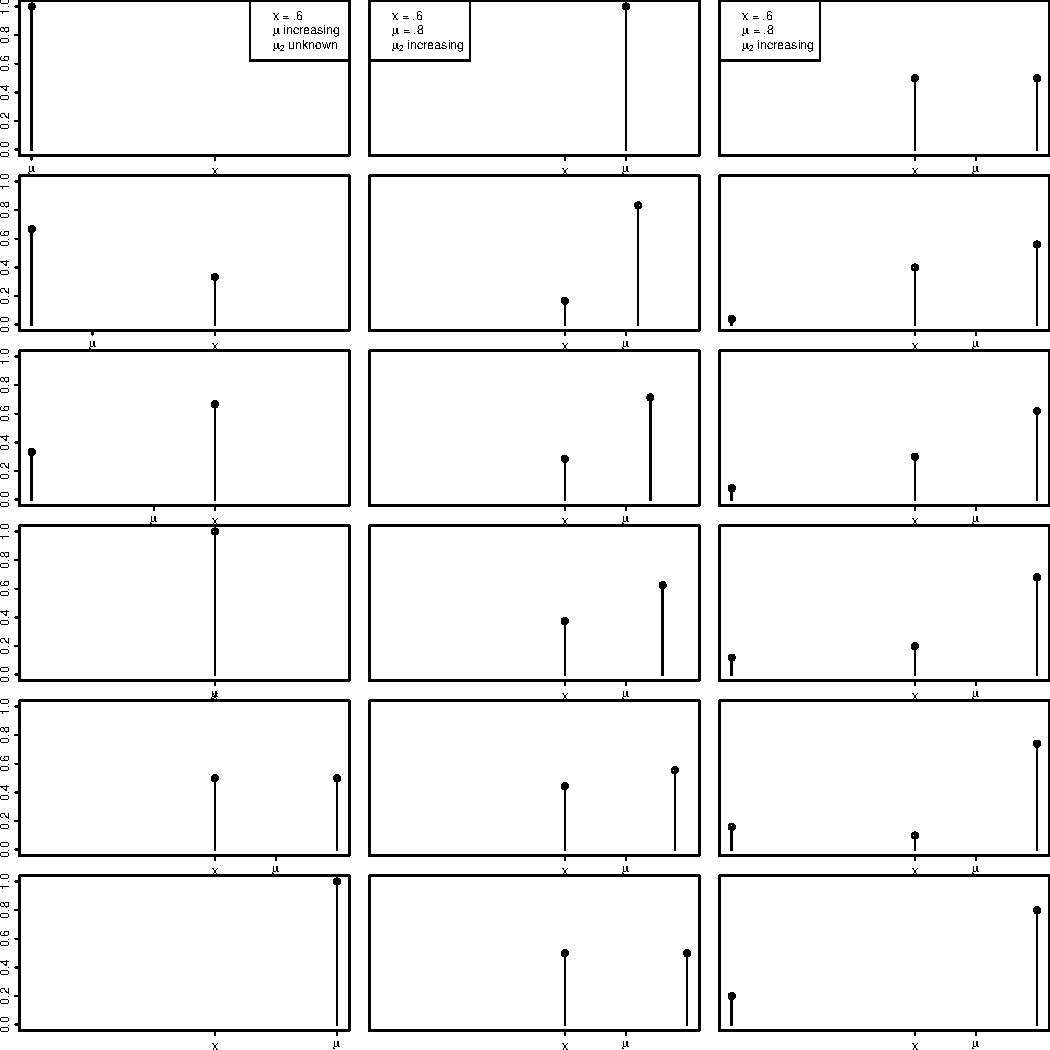
\includegraphics[width=\linewidth]{densities.pdf}
\caption{Distributions that minimize $\Fmin$ and maximize $\Fmax$.
The left column has $\mu_2$ unknown ($F_2$ and $F_1$).
The middle column has variance increasing from 0 to $\sigma_*^2$ ($F_3$).
The right column has variance increasing from $\sigma_*^2$ to the
maximum ($F_4$).
\label{fig:densities}
}
\end{figure}


The EMDCC is the integral of the difference between upper and lower
bounds, given by $p_1$ or $p_2$:
\begin{eqnarray}
  \mbox{EMDCC}
  &=& \int_0^1 \Fmax(x) - \Fmin(x) du \nonumber \\
  &=& \int_0^\mu p_1 dx + \int_\mu^1 p_2 dx \nonumber \\
  &=& \int_0^\mu (1-\mu)/(1-x)dx + \int_\mu^1 1 - (1 - \mu/x) dx \nonumber \\
  &=& -(1-\mu) \log(1-\mu) - \mu \log(\mu)
\end{eqnarray}

% plot(function(mu)  -(1-mu) * log(1-mu) - mu * log(mu))
% abline(h = 1/2)
% uniroot(function(mu)  -(1-mu) * log(1-mu) - mu * log(mu) - 1/2, c(.1, .3))


The EMDCC approaches 0 for $\mu$ near 0 or 1, and has a maximum value
of $\log(2) = .69$ when $\mu = 1/2$. This EMDCC is smaller than for
a non-polynomial histogram with twice as many bins
for $0 \le \mu < 0.1997$ or $0.8003 < \mu \le 1$.

\begin{theorem}
$F_1$ and $F_2$ minimize $F_{-}(x)$ and maximize $F(x)$,
for $x \le \mu$ and $x \ge \mu$, respectively.
\end{theorem}

\begin{proof}
The case $x = \mu$ is trivial; both $F_1$ and $F_2$ reduce to
$F_x$, the distribution with a point mass at $x$, which optimizes
both objectives.

Consider the case with $x < \mu$; we claim that $F_1$ given above is optimal,
with density (point mass) $f^*(x) = p_1$
and $f(1) = 1-p_1$, and zero elsewhere.
This has the minimum possible lower bound $F_{1-}(x) = 0$,
so consider the upper bound.

Suppose some other distribution $F$ has mass elsewhere.
Then
\begin{eqnarray}
  \mu
  &=& \int_0^1 u dF(u) \\
  &=& \int_0^{x-} u dF(u) + x P(X=x) + \int_{x+}^{1-} u dF(u) + P(X=1) \\
  &<& \int_0^{x-} x dF(u) + x P(X=x) + \int_{x+}^{1-} 1 dF(u) + P(X=1) \\
  &=& x F(x) + 1 - F(x)
\end{eqnarray}
Solving for $F(x)$ gives $F(x) < (1-\mu) / (1-x) = p_1$,
which is inferior to $F_1(x)$.

The case with $x > \mu$ is similar; $F_2$ is optimal for both
$\Fmin$ and $\Fmax$.
The solutions for this case can be obtained from the previous using
$X' = 1-X$,
$x' = 1-x$, and
$\mu' = 1 - \mu$.

When $x = \mu$, both $F_1$ and $F_2$ simplify to a point mass at $\mu$.
\end{proof}


\subsection{Second Moment}

Now suppose that the first two moments are known.
For any value of $x$, we seek distributions that minimize
$F_{-}(x)$ and maximize $F(x)$, to determine $\Fmin$ and $\Fmax$.
As before, surprisingly, a single distribution
does both---the distribution that places maximum mass at $x$, subject
to the moments.

As before, there are two cases. It is easiest to
think of these as the ``small variance'' and ``large variance'' cases,
though they also correspond to values of $x$.
Let $\sigma^2 = \mu_2 - \mu^2$.
Let $\mu_2^*$ be the second moment for $F_1$ or $F_2$, for
$x \le \mu$ or $x > \mu$ respectively, and
$\sigma_*^2$ be the corresponding variance.
We can also write $\sigma^{*2}$ as
$\sigma_{F_1}^2 = (1-\mu)(\mu-x)$
or
$\sigma_{F_2}^2 = (x-\mu)(x - 0)$, respectively.

% May eliminate some of that notation if I don't use it.

There are three sub-cases to consider:
$\mu_2 < \mu_2^*$,
$\mu_2 > \mu_2^*$, and
$\mu_2 = \mu_2^*$.
The third case is trivial, the solution is the same as for $\mu_2$ unknown,
either $F_1$ or $F_2$.

Consider the small variance case, with $\mu_2 < \mu_2^*$.
Recall that $F_1$ places mass at $x$ and $1$,
and $F_2$ at $0$ and $x$.
With smaller $\mu_2$ (and smaller variance), the optimal solution
is again a two-point distribution,
with support at $x$ and $a$.
Solving the moment equations gives
$a = \mu + \sigma^2/(\mu-x)$,
with $P(X = x) = p_3 = \sigma^2 / (\sigma^2 + (\mu-x)^2)$ and
$P(X = a) = 1-p_3$.
We call this distribution $F_3$ below.
It reduces to either $F_1$ or $F_2$
(i.e.\ $a=1$ or $a=0$) when $\mu_2 = \mu_2^*$.
As $\sigma^2$ shrinks, $a$ moves from $0$ or $1$ toward $\mu$,
and mass moves from $x$ to $a$.

\begin{theorem}
For $\mu_2 < \mu_2^*$,
$F_3$ maximizes $F(x)$ and minimizes $F_{-}(x)$, subject to $\mu$
and $\mu_2$.
\end{theorem}

In particular,
for $x < \mu$, $F_3$
has $F_{-}(x) = 0$ (the smallest possible) and
$F(x) = p_3$, the largest possible given the constraints.
For $x > \mu$, $F_3$
has $F(x) = 1$ (the largest possible) and
$F_{-}(x) = f_x$, the smallest possible given the constraints.
This case ($\mu_2 < \mu_2^*$) does not occur when $x = \mu$.

\begin{proof}
We consider the case with $x < \mu$.
For any $F$, the first two moments can be decomposed as
\begin{eqnarray}
  \mu &=& \int_0^x u dF(u) + \int_{x+}^1 u dF(u) \nonumber \\
      &\le& x F(x) + \int_{x+}^1 u dF(u) \nonumber \\
  \sigma^2 &=& \int_0^x (u-\mu)^2 dF(u) + \int_{x+}^1 (u-\mu)^2 dF(u) \nonumber\\
       &\le& (x-\mu)^2 F(x) + \int_{x+}^1 (u-\mu)^2 dF(u) \nonumber
\end{eqnarray}
with equality if $P(X < x) = 0$.
From the first inequality we get
$\int_{x+}^1 u dF(u) \ge \mu - x F(x)$, so
the conditional mean satisfies $E(X | X > x) \ge (\mu - x F(x))/(1-F(x)$.
Second,
$$\int_{x+}^1 (u-\mu)^2 dF(u) \le \sigma^2 - (x-\mu^2) F(x).$$
But from the conditional mean and Jensen's inequality we have
\begin{eqnarray}
  \int_{x+}^1 (u-\mu)^2 dF(u)
  &\ge& (E(X | X > x) - \mu)^2P(X > x) \nonumber \\
  &\ge& \left( \frac{\mu-x F(x)}{1-F(x)} - \mu\right)^2 (1-F(x)) \nonumber \\
  &=& F(x)^2 (\mu-x)^2 / (1-F(x)) \nonumber
\end{eqnarray}
with equality
if $F$ has conditional variance zero for $X > x$ and $P(X < x) = 0$.

Combining inequalities, we have
$F(x)^2 (x-\mu)^2 / (1-F(x)) \le \sigma^2 - (x-\mu^2) F(x)$
with equality if $F$ has two point masses, one at $x$.
This simplifies to
$$ F(x) \le \sigma^2 / (\sigma^2 + (x - \mu)^2) = F_{1A}(x).$$
Hence no other distribution can have larger $F(x)$.

The case with $x > \mu$ is similar.
\end{proof}

For the large variance case,
with $\mu_2 > \mu_2^*$,
the variance is larger than $\sigma_*^2$,
and as the variance increase
the optimal solution moves mass
from $x$ to $0$ and $1$.
Let $F_4$ be the distribution with mass at $0$, $x$, and $1$ that
satisfies the two moment constraints; this gives
$F_4(x) = p_4 = (\mu-\mu_2)/(x-x^2)$,
$F_4(1) = \mu - x p_4$, and
$F_4(0) = 1 - p_4 - F_4(1)$.

\begin{theorem}
For $\mu_2 \ge \mu_2^*$,
$F_4$ maximizes $F(x)$ and minimizes $F_{-}(x)$, subject to $\mu$
and $\mu_2$.
\end{theorem}

\begin{proof}
For any $F$,
suppose there is mass between $0$ and $x$.
Then move that mass to 0 and 1, while keeping the same mean
(If $b$ is the conditional mean given $0 < X < x$, then move
fraction $b/x$ of the mass to $x$ and the rest to $0$).
Similarly, if there is mass between $x$ and $1$, move that
mass to $x$ and $1$ while keeping the same mean.
Call the resulting distribution $F'$; it has the same mean and
larger variance than $F$,
and objective functions that are at least as good:
$F_{-}'(x) \le F_{-}(x)$ (with equality if $F$ has no mass in $(0,x)$)
and
$F'(x) \ge F(x)$ (with equality if $F$ has no mass in $(x,1)$).

The objective functions can be further improved by reducing
the variance to the desired value, using a linear combination of $F'$
and $F_x$.
Let $F'' = \lambda F' + (1-\lambda) F_x$,
where
% $F_x$ is the distribution with a point mass at $x$ and
$\lambda = \sigma^2 / \sigma^2_{F'}$.
$F''$ has moments $\mu$ and $\mu_2$
and objective functions
$F_{-}''(x) = \lambda F_{-}'(x) < F_{-}(x)$
and
$F''(x) = \lambda F'(x) + (1-\lambda) > F(x)$.
In other words, if a distribution has mass anywhere other than $0$, $x$,
and $1$, both objective functions can be improved.
Hence $F_4$, the only distribution with mass at only those three points
that satisfies both moment conditions, is optimal.
\end{proof}

We earlier expressed the boundary between small and large variance
cases according to whether $\sigma^2 < \sigma_*^2$.
For $x < \mu$ this simplifies to $x < c_1 = \mu - \sigma^2 / (1-\mu)$
and for $x > \mu$ it simpifies to $x > c_2 = \mu + \sigma^2 / \mu$.
In other words, the large variance case occurs when
$c_1 \le x \le c_2$,
and the small variance case when $x$ is outside these bounds.

The distributions are summarized in Table~\ref{table:optimalDistributions}.
These distributions are summarized in the first two cases in
Table~\ref{table:optimalDistributions}
and shown in the left column of
Figure~\ref{fig:densities}.
The lower and upper bounds $\Fmin$ and $\Fmax$ are shown
in Figure~\ref{fig:bounds}.


The EMDCC is the integral of the difference between upper and lower
bounds; the difference is given by $p_3$ or $p_4$:
\begin{eqnarray}
  \mbox{EMDCC}
  &=& \int_0^1 \Fmax(x) - \Fmin(x) du \nonumber \\
  &=& \int_0^{c_1} p_3 dx + \int_{c_1}^{c+2} p_4 + \int_{c_2}^1 p_3 dx\nonumber \\
  &=& |_0^{c_1} P_3 + |_{c_1}^{c+2} P_4 + |_{c_2}^1 P_3 \nonumber \\
\end{eqnarray}
where $P_3 = \sigma \tan^{-1}((x-\mu)/\sigma)$ and
$P_4 = (\mu - \mu_2)\log(x/(1-x))$ are antiderivatives of $p_3$ and $p_4$.


\begin{figure}
\centering
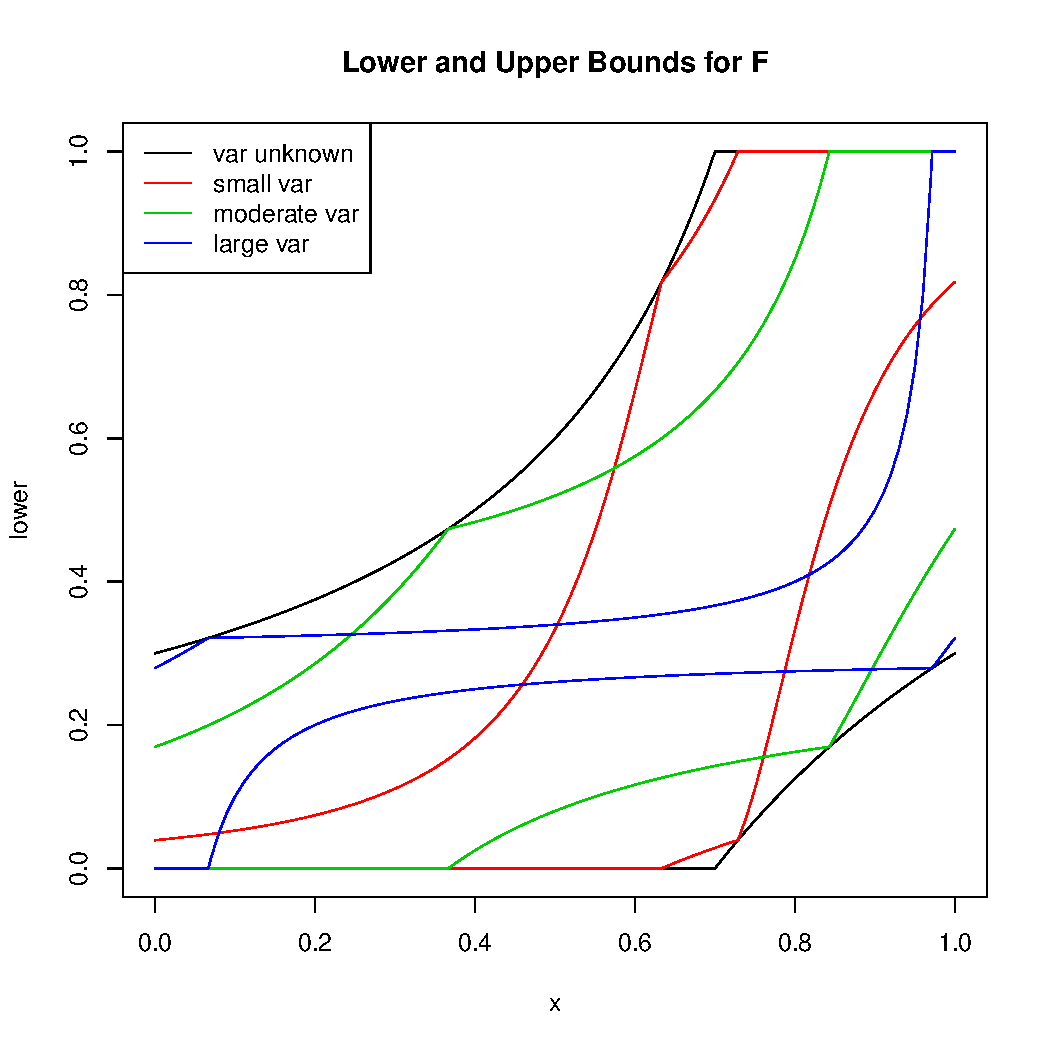
\includegraphics[width=\linewidth]{bounds.pdf}
\caption{Lower and upper bounds $\Fmin$ and $\Fmax$, for $\mu$
unknown and small, middle and large variances.
\label{fig:bounds}
}
\end{figure}


% The cutoff between the $F_3$ and $F_4$ cases nominally depends on
% whether $\mu_2 < \mu_2^*$, but $\mu_2^*$ is a function of $x$,
% so we can express the cutoff as a function of $x$.
% The cutoffs are shown in Table~\ref{table:optimalDistributions}.
% Here is an explanation of what values of $x$ lead to the
% different cases.
%
% For $x$ near zero or one, in particular for
% $0 < x < c_1$
% or
% $c_2 < x < 1$,
% the variance $\sigma_*^2$ of
% $F_1$ or $F_2$ is large,
% $\sigma^2 < \sigma_*^2$, and the $F_3$ distribution applies.
%
% Conversely, for $x$ near $\mu$, $c_1 < x < c_2$,
% the variance $\sigma_*^2$ of
% $F_1$ or $F_2$ is small,
% $\sigma^2 > \sigma_*^2$, and the $F_4$ distribution applies.
% $F_4$ increases the variance to $\sigma^2$ my moving
% some mass from $x$ to $0$ and $1$.








%------------------------------------------------------------
\section{Old material}

Below is from polyhist.tex, sections 2.1-2.2, with minor fixes.
Some of this duplicates the above.
I'm including this here in case we want to include some of the older text,
in order to not lose the fixes.


In evaluating representations of system distributions, we define the
\emph{Earth Mover's Distance of the Cumulative Curves} (EMDCC) as our information
loss metric.  In particular, if $X$ is the (unknown) underlying data set with
distribution $F$, and $h$ is our data representation, r is the range of our representation,
then we define upper and lower bounds $F_{h+}(x) \quad F_{h-}(x)$ as the highest and lowest possible
values for the true distribution given the observed representation, and the
EMDCC as the normalized L1 distance between them:

$$ \mbox{EMDCC}(X, h) = \frac{1}{r}
    \int_{\mathbb{R}} | F_{h+}(x) - F_{h-}(x) |dx $$

\noindent noting that in the case that $h$ is a histogram bucketing scheme,
$F_{h-}$ always puts its mass on the right endpoints and $F_{h+}$ always puts
near the left endpoints.  The Earth Mover's Distance
\cite{rubner2000earth} is also known as the
Mallows distance, or Wasserstein distance with $p=1$ in
different communities.

Figure~\ref{fig:emdcc} shows a histogram (left) along with the CDF representation and the
associated area of uncertainty (in yellow).  Any underlying dataset
having the given histogram representation must have a true ecdf lying
entirely within the yellow area.  A histogram with more granular
buckets would reduce the information loss at the expense of additional
storage space to store the buckets.

\begin{figure}[h!]
\centering
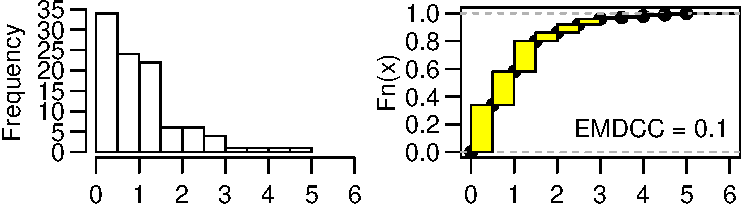
\includegraphics[width=\linewidth]{exhists-crop.pdf}
\caption{An example histogram (left) with its CDF representation and a
  yellow area of uncertainty showing where the true empirical cdf of
  the unbinned data must lie (right).}
% \label{fig:emdcc}  % I defined this figure above.
\end{figure}

% We say this where we need it in emprical validation section, no
% space to say it twice.
%We assume bucket boundaries are stored separately
%so that histograms are represented as simply an array of integers representing
%the counts of each bucket.
Adding more buckets as in this example usually reduces the EMDCC, but
are there more efficient ways to reduce the EMDCC for a given amount
of storage space?

\subsection{Polynomial Histograms}

Given a fixed amount of storage space, we can trade off the granularity of
histogram buckets for additional statistics within each bucket.  For example,
in addition to storing the counts between histogram boundaries $(a, b)$, we
could also store the mean and higher moments.  Histograms with
annotations of moments per bin are known as \emph{Polynomial
Histograms} \cite{sagae1997bin}.  Storing the moments is appealing in
a distributed systems context because merging histograms with the same
bucket boundaries remains trivial.  We will use the notation $H(b,p)$ to
denote a histogram with $b$ bins annotated with the $p$-moments of
each bin.

Knowing the first moment can help a lot when it is near the boundary; the
EMDCC associated with bucket $(a, b)$ will be zero if the mean is $a$.
%More generally, assume that we track the $p^{th}$ moment within each bucket $(a,b)$, where
%$$ \mu_p = (\frac{1}{N} \sum_{i=1}^N x_i^p)^{\frac{1}{p}} $$
%Then letting $\alpha = \frac{b^p - \mu_p^2}{b^p - a^p}$ implies that the EMDCC will decrease
%from it's original area by a factor of:
In general, with many points in bucket, a continuous approximation says that a mean of $\mu = \alpha * a + (1-\alpha) * b$ gives an EMDCC of

$$
\lambda(\alpha) = \alpha * ln(\frac{1}{\alpha}) + (1 - \alpha) * ln(\frac{1}{1-\alpha})
$$

The function $\lambda(\alpha)$ is symmetric around $0.5$, is increasing up to it's max of $\lambda(0.5) \approx 0.7$, integrates to $0.5$, and $\lambda(0.2) = \lambda(0.8) \approx 0.5$.  Since bisection always halves the EMDCC, this gives rules of thumb about the merits of bisection vs. storing the mean; if $\alpha < 0.2$ or $\alpha > 0.8$ then storing the mean is better, storing the mean can be worse than bisection by 40\% but it can also be infinitely better, if $\alpha's$ are uniformly distributed and independent of the counts per bucket then bisection and storing the mean should give the same reduction on average.  If the true density is smooth enough relative to the bucketing scheme, then $\alpha$ will tend to be closer to $\frac{1}{2}$, which implies inferiority of keeping the mean with respect to the EMDCC metric.


\noindent
\textbf{Proof:} \\

We restrict our attention to $(a,b)$ where we also know the $p^{th}$ moment$\big(\mu_p^p = \frac{1}{n} \sum_{i=1}^n x_i^p \big)$.  We construct $F_{h+}(x), F_{h-}(x)$ pointwise as the upper and lower bound curves, then integrate to find the reduction in EMDCC. % (only maybe use)  For convenience, we define $\alpha_p = \frac{b^p-\mu_p^p}{b^p-a^p}$

For $x \in (a, \mu_p)$, the lower bound is $F(a)$ and the upper bound has support $\{x, b\}$.  This implies that $\mu_p^p$ equals

$$
\frac{F_{h+}(x)-F(a)}{F(b)-F(a)} * x^p + \frac{F(b)-F_{h+}(x)}{F(b)-F(a)} * b^p
$$

Therefore,

$$
F_{h+}(x) = F(a) + (F(b)-F(a)) \frac{b^p-\mu^p}{b^p-x^p}
$$

For $x \in (\mu_p, b)$, the upper bound is $F(b)$ and the lower bound has support $\{a+\epsilon, x+\epsilon\}$ where we let $\epsilon \rightarrow 0$.  This implies that $\mu_p^p$ equals

$$
\frac{F_{h-}(a+\epsilon)-F(a)}{F(b)-F(a)} * (a+\epsilon)^p + \frac{F_{h-}(x+\epsilon)-F_{h-}(a + \epsilon)}{F(b)-F(a)} (x + \epsilon)^p
$$

Therefore, re-arranging, noting that $F_{h-}(a+\epsilon)=F_{h-}(x)$, $F_{h-}(x+\epsilon)=F(b)$, and letting $\epsilon \rightarrow 0$ gives

$$
F_{h-}(x) = F(b) - (F(b)-F(a)) \frac{\mu_p^p - a^p}{x^p-a^p}
$$

Next, the area reduction from knowing the moment comes from the integral between upper and lower bounds:

$$
\frac{1}{(F(b)-F(a))(b-a)}\int_{a}^{b} |F_{h+}(x) - F_{h-}(x)|dx =
$$
$$
\frac{1}{b-a} \bigg(
\int_{a}^{\mu_p} \frac{b^p-\mu_p^p}{b^p-x^p}dx + \int_{\mu_p}^{b} \frac{\mu_p^p-a^p}{x^p-a^p}dx
\bigg)
$$

\noindent
and this gives the stated result when $p=1$.  More complex formulas exist when multiple moments are known simultaneously.

Figure~\ref{fig:polyemdcc} uses an example bin with points taken from
Beta(0.5, 0.05) and a mean value of 0.9 to illustrate visually the
tradeoff in information loss between $H(2,0)$ and $H(1,1)$ histograms.
Knowing the mean value in this case
constrains the area where an ecdf of the underlying distribution with
that binned representation lies more than if we had just added twice
as many bins at the same storage cost.

\begin{figure}[h!]
\centering
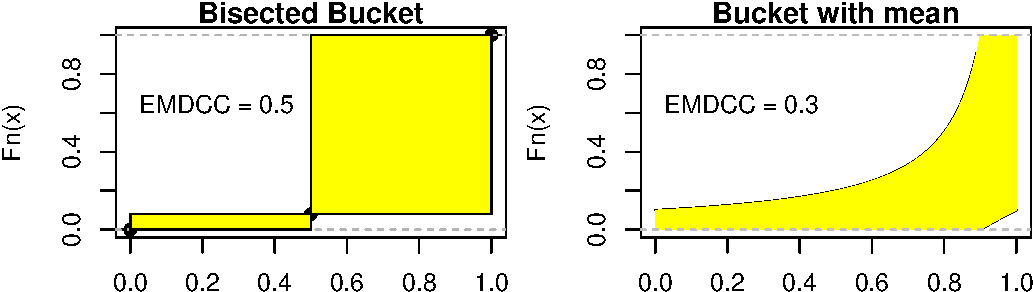
\includegraphics[width=\linewidth]{polyhistemdcc-crop.pdf}
\caption{Yellow areas of uncertainty for where the ecdf of the
  unbinned data must lie given a histogram bin bisected in two (left)
  or a histogram annotated with the mean of values in that bin (right).}
\label{fig:polyemdcc}
\end{figure}

\end{document}


% C-c > is mapped to reftex-display-index
% C-c - was mapped to reftex-toc-recenter
% I mapped them in .emacs (reftex-mode-hook) to string-rectangle & dashes

% (reftex-mode nil)
% (reftex-mode t)

% open -a /Applications/Preview.app ~/consulting/MurrayStokely1404/paper/proof.pdf
